%!TEX root = /Users/jakubkonka/Thesis/Thesis.tex
\chapter{Intelligent Network Selection} % (fold)
\label{cha:intelligent}

\minitoc
\vspace{10mm}

\section{The Problem of Intelligent Network Seletion} % (fold)
\label{sec:the_problem_of_intelligent_network_seletion_intelligent}
The aim of this section is to explain the concept and importance of intelligent network selection in the future wireless access networks. To this end, this section starts with an explanation of the concept of a heterogeneous wireless access network. It then moves onto a discussion of the Always Best Connected paradigm and the role of intelligent network selection in fulfilling its assumptions. Finally, the importance of economic aspects of intelligent network selection is highlighted.

\subsection{Heterogeneous Wireless Access Network} % (fold)
\label{sub:heterogeneous_wireless_access_network_intelligent}
Over the last decade, the world of wireless and mobile communications has witnessed several major improvements \cite{ABC03}. The evolution of traditional 2$^\text{nd}$ Generation (2G) cellular systems (such as GSM), through 3$^{\text{rd}}$ Generation (3G) systems (such as UMTS or CDMA2000), into 4$^{\text{th}}$ Generation (4G) systems (such as LTE), has drastically improved the cellular coverage worldwide, and provided mobile Internet access \cite{HossainBeaubrun09, HossainTalebiFard09}. At the same time, IEEE 802.11-based Wireless Local Area Network (WLAN; commonly referred to as WiFi) solutions have emerged as the predominant high-speed wireless Internet access at airports, in hotels, or even at home.

With the introduction of smartphones (iPhones, Android phones, BlackBerry phones) and tablets (iPads, Android tablets), the wireless users are finally able to take advantage of both the coverage offered by 3G/4G cellular access network and the high-speed Internet access offered by WiFis. Whenever the smartphone/tablet is in close proximity to a WiFi hot spot, it automatically switches from 3G/4G to WiFi mode for faster data access. However, this only works when either the WiFi hot spot provides free access, or is within the user's subscription; for example, as part of the monthly data allowance plan with a local wireless access network operator. Moreover, this solution lacks the support for session continuity, and does not provide any intelligence when switching from one access network to another. For instance, although the WiFi hot spot is by definition deemed to offer faster data rates, this does not necessarily translate into higher Quality of Service (QoS). In fact, it might be just the contrary, especially in a very crowded hot spot area where the users run very bandwidth intensive applications such as video or music streaming, or even on-line gaming. For example, under such circumstances, trying to make a Skype call can be nearly impossible \cite{Wisely4gWLAN09}. Therefore, the decision to switch from one network to another should not only consider the availability of a particular wireless access network, but also the offered QoS for the best user experience.

\begin{figure}[t]
    \centering
    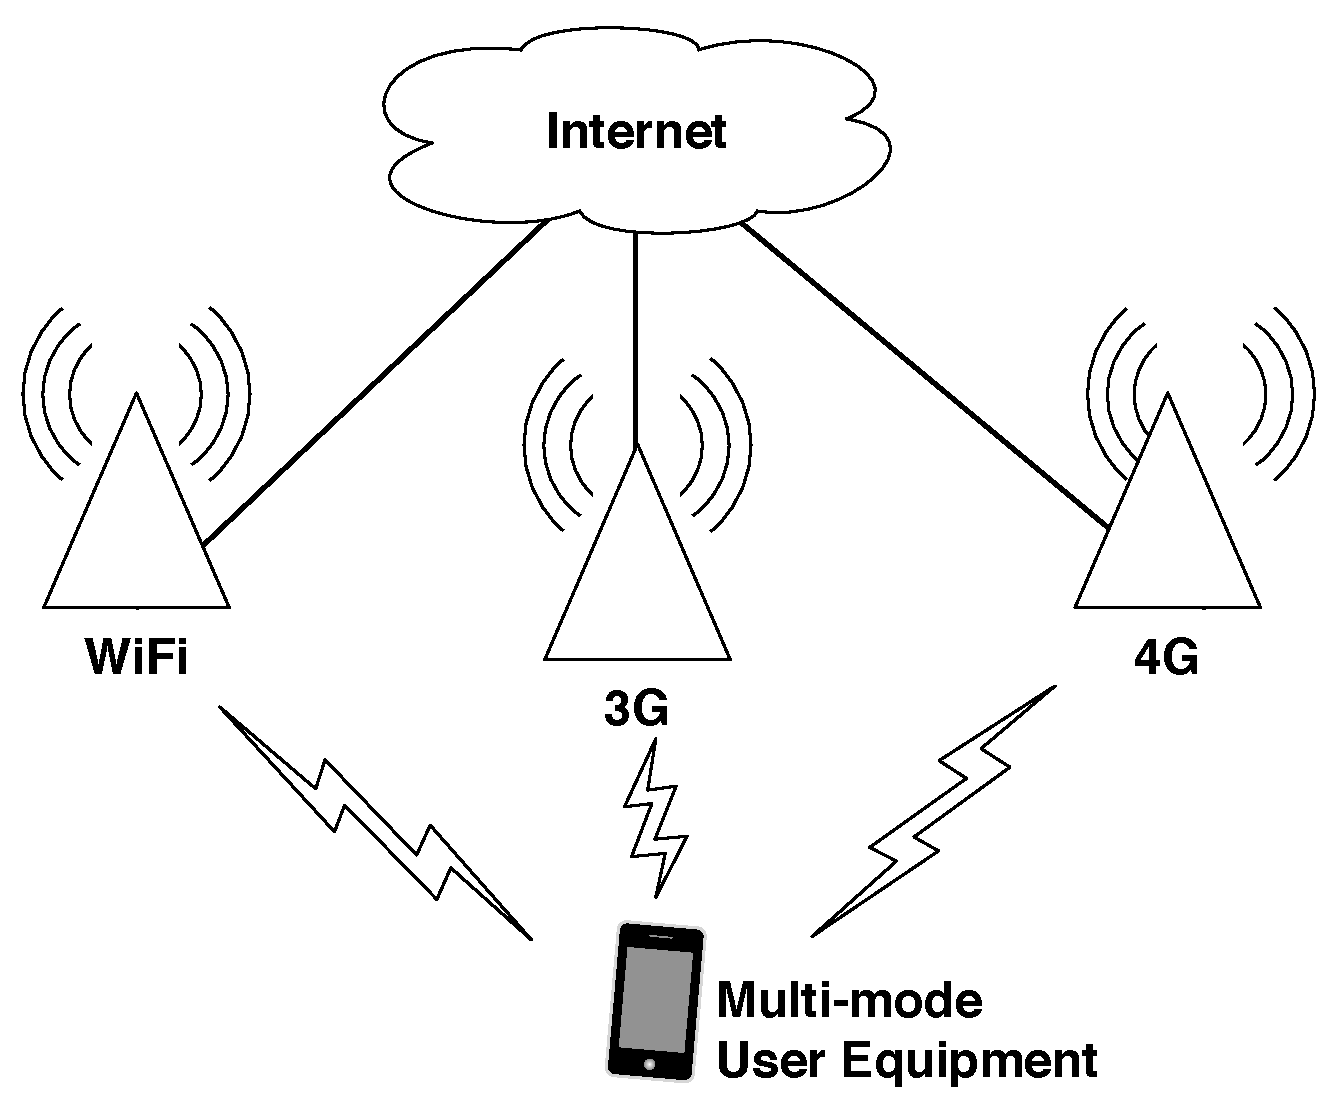
\includegraphics[width=3.5in]{Intelligent/Figures/heterogeneous}
    \caption{Heterogeneous wireless access network}
    \label{fig:heterogeneous_intelligent}
\end{figure}

This, together with the industry's drive to have an all-IP-based traffic, gives rise to the concept of a \emph{heterogeneous wireless access network}. The heterogeneous wireless access network spans different wireless access technologies integrated into one network to provide wireless and mobile users with the requested multimedia services and QoS. It will take full advantage of the multi-modality offered by the smartphones by having the device connected to all wireless access technologies at all times. This is depicted in Figure~\ref{fig:heterogeneous_intelligent}.

The heterogeneous wireless access network will possess many advantages over the contemporary wireless networking solution. From the users' perspective, different coverage and QoS characteristics of each of the included wireless access technologies will lead to the ability to seamlessly connect at any time, at any place, and to the access technology which offers the most optimal quality available. This is referred to as \emph{Always Best Connected} paradigm \cite{ABC03}, and will be introduced in more detail in the subsequent section. From the network operators' perspective, on the other hand, the integration of wireless access technologies will allow for more efficient usage of the network resources, and might be the most economic way of providing both universal coverage and broadband access \cite{HossainBeaubrun09}.

\begin{figure}[t]
    \centering
    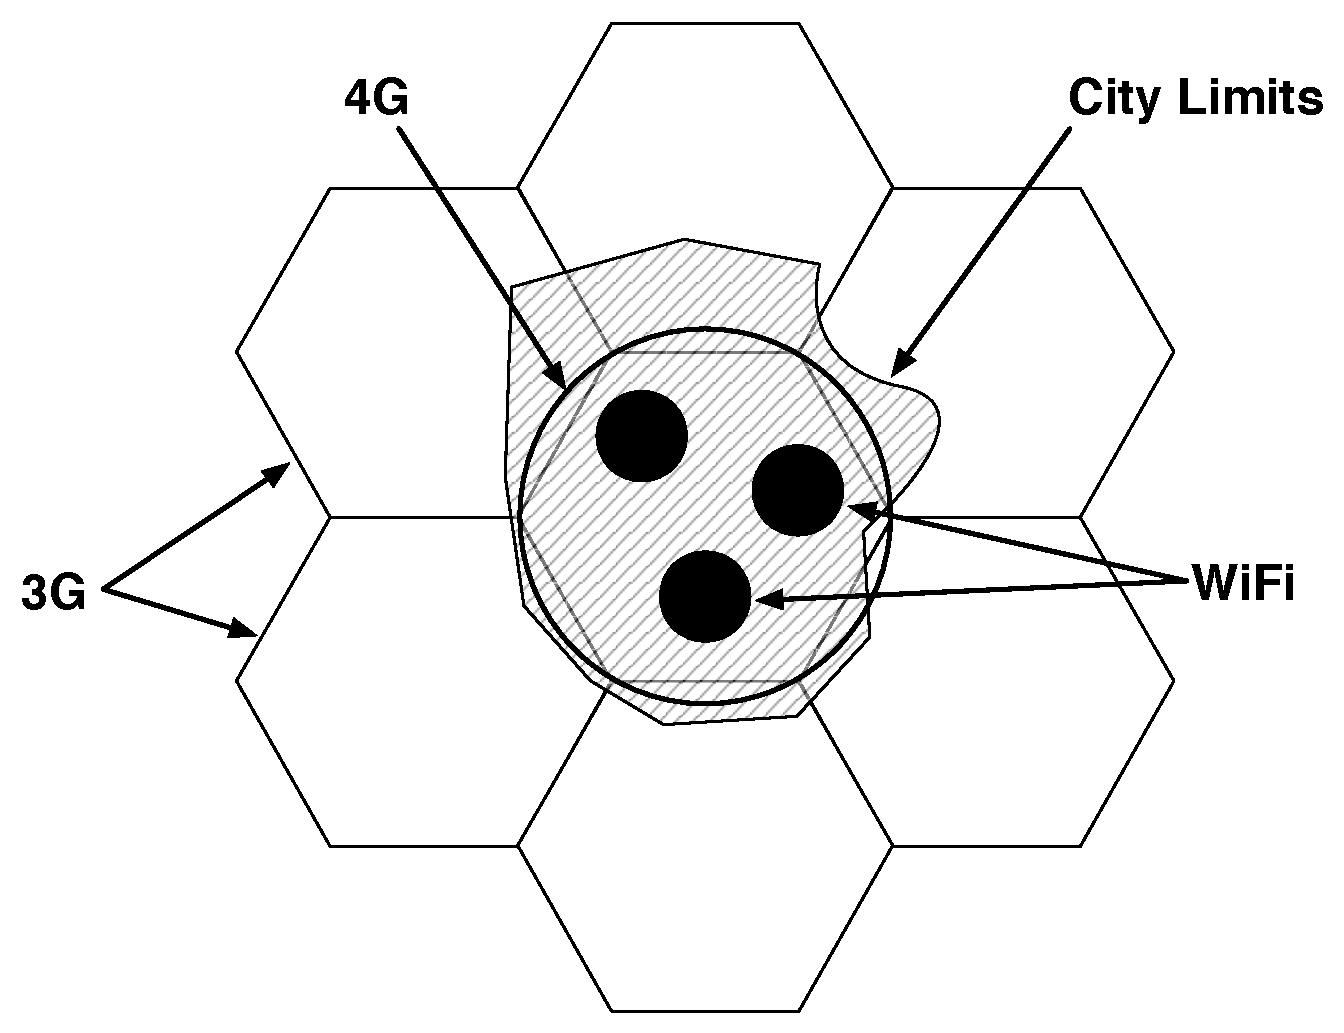
\includegraphics[width=4in]{Intelligent/Figures/wireless_city}
    \caption{Typical distribution of wireless access technologies in a modern-day city}
    \label{fig:wireless_city_intelligent}
\end{figure}

Figure~\ref{fig:wireless_city_intelligent} depicts a typical distribution of wireless access technologies in a modern-day city. In the example, WiFi hot spots are used as a localised very high-speed Internet access; 4G covers nearly the $\sfrac{3}{4}$ of the city area, and provides high-speed Internet access; and 3G delivers medium speed wireless access inside as well as outside the city. There is a high overlap of different wireless access technologies within the city. With the adoption of a heterogeneous wireless access network, this overlap could be utilised to its full potential by providing better network resources management, and high-speed and high quality Internet access for the users inside as well as outside the city limits.
% subsection heterogeneous_wireless_access_networks (end)

\subsection{Always Best Connected and Intelligent Network Selection} % (fold)
\label{sub:always_best_connected_and_intelligent_network_selection_intelligent}
As briefly mentioned in the previous section, \emph{Always Best Connected (ABC)} paradigm assumes that a wireless user is: (1) ``always'' connected to the Internet, and (2) uses the ``best'' access technology available \cite{ABC03}. ``Always'' should be interpreted as being able to utilise all wireless access technologies available at any time, while ``best'' implies that when a particular technology is being chosen, several factors such as user preferences, application requirements, network coverage, etc., are considered in order to make the most optimal selection possible (Figure~\ref{fig:abc_intelligent}). The mechanism responsible for implementing the ABC principles is referred to as \emph{intelligent network selection}.

\begin{figure}[t]
    \centering
    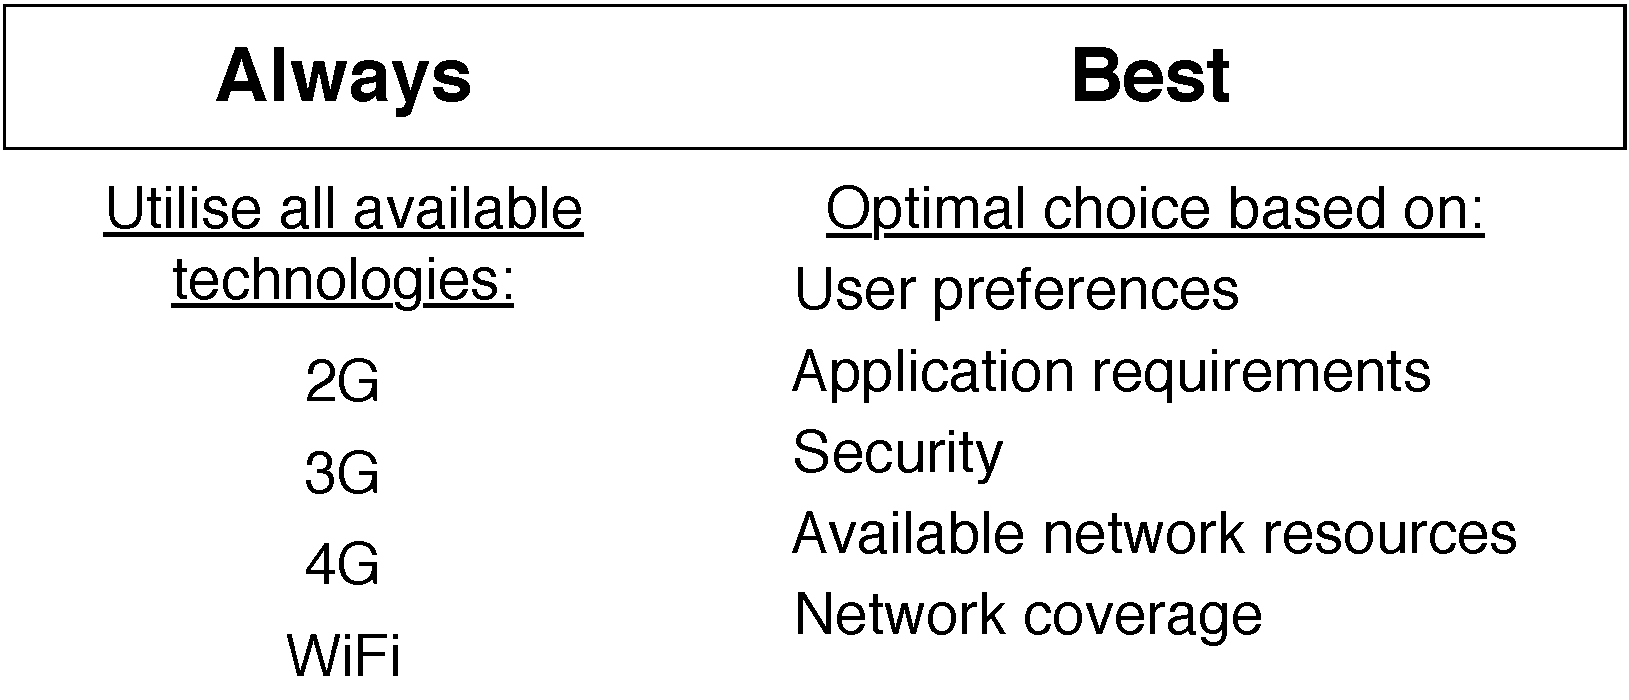
\includegraphics[width=4in]{Intelligent/Figures/abc}
    \caption{The essence of ABC networking paradigm}
    \label{fig:abc_intelligent}
\end{figure}

Furthermore, the paradigm emphasises seamless information delivery and extensive mobility support. In other words, the changes in the communications environment should affect the user as little as possible, even when they are ``on the move''. Therefore, should the user move from the coverage area of one access technology to another, the switch should be as non-disrupting for the user as possible; i.e., the session continuity should be maintained at all times, regardless of the access technology currently used. Thus, it is clear that intelligent network selection plays a vital role in the successful operation of the ABC solution.
% subsection always_best_connected_networking_paradigm (end)

\subsection{Economic Aspects of Intelligent Network Selection} % (fold)
\label{sub:economic_aspects_of_intelligent_network_selection_intelligent}
While the integration of wireless access technologies into the heterogeneous wireless access network will lead to more efficient usage of network resources, the network operators will also be required to cooperate closely in order to manage such a complex system~\cite{HossainBeaubrun09,HossainTalebiFard09}. For example, new service agreements will need to be drafted to enable roaming access for users from and to the other network operators' networks.

Furthermore, since there are many different actors with opposing interests involved, there also exists the possibility of a `tussle'~\cite{Clark02}. For example, it is in the best interest of the users to obtain the highest quality of the service for the lowest price. Network operators, on the other hand, aim to maximize their profit by performing efficient load balancing. Furthermore, the situation may become even more complex should the service provision be decoupled from the network operators; that is, if the service provision is handled by a separate entity, service provider, while network operators are left with handling of the transport provision~\cite{DMBushTussle09}. Therefore, the problem of intelligent network selection, which as pointed out in the previous section, was considered to be technologically difficult, can also be considered to be the problem of economics where wireless access, traded on a per connection basis, is an electronic good that is sold to the users.

The next section summarises the research efforts of the researchers on the problem of intelligent network selection.
% subsection economic_aspects_of_intelligent_network_selection (end)
% section the_problem_of_intelligent_network_seletion_intelligent (end)

\section{Intelligent Network Selection in the Literature} % (fold)
\label{sec:intelligent_network_selection_in_the_literature_intelligent}
Over the last decade, several papers have explored the problem of intelligent network selection in heterogeneous wireless access networks. It is the aim of this section to summarise the research work of other researchers on the problem of intelligent network selection. To this end, we group the approaches based on their mathematical underpinnings; that is, we discuss utility theory based approaches, multiple attribute decision making, fuzzy logic, game theory, combinatorial optimisation, and other. The grouping is based on an excellent survey paper by Wang and Kuo~\cite{LushengKuo2013}.

\subsection{Utility Theory} % (fold)
\label{sub:utility_theory_intelligent}
The utility theory approach to network selection is based on the concepts of classical demand theory of microeconomics. Classical demand theory assumes that each consumer is characterised by a preference relation that can be captured by a mapping into real numbers---the utility function~\cite{MicroTheory}. For example, suppose a consumer prefers a monthly subscription contract to wireless services over a yearly one. Then, their utility of the former is greater than the utility of latter.

When applied to the problem of intelligent network selection, the main challenge is to capture mobile users' preferences for different attributes/characteristics of a wireless service in the form of utility functions~\cite{LushengKuo2013}. Some common attributes include but are not limited to: bandwidth required by the service, price of the service, bit error rate, delay, etc. However, the main challenge of the approach is also its main shortcoming, since as discussed by Wang and Kuo~\cite{LushengKuo2013}, there are as many characterisations of the attributes and associated utility functions as there are researchers working on the problem of utility-based network selection (cf.~Table III in~\cite{LushengKuo2013}).

In its simplest form, the network selection mechanism uses the derived utility functions for different attributes to select network/access technology that yields the highest overall utility to the user. A more interesting approach, however, proposed by Ormond \emph{et al.}~\cite{OrmondCS106,OrmondCS206,OrmondCS306} utilises the concept of consumer surplus to drive network selection. In economic terminology, consumer surplus refers to a measure of net benefit from consuming a good, and is equal to the difference between the utility the consumer extracts from consuming the good and its price~\cite{MicroTheory,Varian2010,Varian1992}. In their work, Ormond \emph{et al.}~focus mainly on non real-time data services, and for this case, derive a non increasing utility function which captures user's willingness-to-pay versus their willingness-to-wait. The network that achieves the highest consumer surplus for the service is then selected.
% subsection utility_theory (end)

\subsection{Multiple Attribute Decision Making} % (fold)
\label{sub:multiple_attribute_decision_making_intelligent}
Multiple attribute decision making (MADM) is a branch of multiple criteria decision making (MCDM), a subdiscipline of operations research~\cite{LushengKuo2013}. The main aim of MADM is to aid a decision-maker in making a complex decision that often depends on multiple, possibly conflicting attributes.

MADM-based network selection is closely related to utility-based approach as it effectively studies methods of combining utilities for different attributes in the most optimal way~\cite{LushengKuo2013}. As such, the main challenge of this approach is similar to that of utility-based approach; that is, capturing user's preference per attribute per scenario.

The MADM-based network selection usually involves~\cite{LushengKuo2013}:
\begin{enumerate}
\item gathering and quantifying values for each considered attribute for each candidate network. For example, candidate network A might have a price attribute of 0.5, while candidate network B of 0.25.
\item calculating weights for each attribute based on user's preferences. For example, user might prefer a higher price but a lower delay, and hence, a higher weight is assigned to the price attribute.
\item utilising a MADM algorithm to score each candidate network based on the combination of attributes and weights. It is interesting to note that the score is equivalent to the combined utility function in the utility-based network selection. The score can be computed, for example, as a simple sum of all the attributes weighted by the weights, or alternatively, the attributes can be raised to the power of the corresponding weights and multiplied together. The former approach is referred to as simple additive weighting (SAW)~\cite{BariLeung2007a}, while the latter as multiplicative exponential weighting (MEW)~\cite{Nguyen2008}. Other popular algorithms include: grey relational analysis (GRA)~\cite{Song2005}, and technique for order preference by similarity to an ideal solution (TOPSIS)~\cite{BariLeung2007b}.
\item selecting candidate network which achieves the highest score.
\end{enumerate}
% subsection multiple_attribute_decision_making (end)

\subsection{Fuzzy Logic} % (fold)
\label{sub:fuzzy_logic_intelligent}

% subsection fuzzy_logic (end)

\subsection{Combinatorial Optimisation} % (fold)
\label{sub:combinatorial_optimisation_intelligent}

% subsection combinatorial_optimisation (end)

\subsection{Markov Chain} % (fold)
\label{sub:markov_chain_intelligent}

% subsection markov_chain (end)

\subsection{Game Theory} % (fold)
\label{sub:game_theory_intelligent}
Game theory deals with the analysis of mathematical models of conflict and cooperation between two or more intelligent individuals~\cite{Myerson97,Gibbons92,Webb07}. In game theoretic terminology, a game refers to any social (and possibly conflictual) situation involving two or more individuals who are referred to as players. The players are assumed to be rational decision-makers; i.e., they will always strive to make the best decision possible in pursuit of their own interests. Furthermore, each player is characterised by a set of strategies and payoffs/utilities for choosing a particular strategy. For each player, payoff depends not only on their chosen strategy, but also on the strategies chosen by other players. The aim of game theoretic analysis is then to characterise an equilibrium (typically, Nash equilibrium); that is, a set of strategies that if played by all the players, guarantee the highest utility given the strategy choices of other players.

There exist two distinct approaches to game theory, classical and evolutionary game theory, and both were extensively applied to the problem of intelligent network selection~\cite{LushengKuo2013}. While classical game theory concentrates on the analysis of possible outcomes of a game between $N$ players, in evolutionary game theory the focus is put on the dynamics of the whole population (or a group) of decision-makers. In other words, classical game theory concentrates on characterising an equilibrium (if exists) to an $N$-player game. Evolutionary game theory, on the other hand, examines how a particular decision made by the whole population changes over time in response to the decisions made by all players individually.

When applied to network selection, the problem is modelled as either a game between the users, or a game between the network operators. As reported by Wang and Kuo~\cite{LushengKuo2013}, there has been research carried out that permitted a third possibility of a game between users and network operators, however, in this thesis, we concentrate mainly on the two former, more widespread approaches.

\subsubsection{Games Between Users} % (fold)
\label{ssub:games_between_users}
Modelling network selection as a game between the users aims at arriving at an (equilibrium) distribution of the users between the available networks, and as a result, avoiding network congestion and performance degradation. In other words, limited wireless resources are shared in the most optimal way between the users, and at the same time, the users select the network that matches their preferences in the best possible way~\cite{Niyato09}. In what follows, we outline a few noteworthy examples of this modelling approach described in the literature.

Niyato and Hossain~\cite{Niyato09} use evolutionary game theory to study dynamics of competition among groups of users in different service areas. The authors propose two algorithms for deriving an equilibrium to the problem: population evolution and reinforcement learning. The first algorithm uses centralised controller (e.g., a base station) to maintain payoff information for all users. In the second approach, each user tries different networks, observes the size of the allocated bandwidth and price from the chosen network, and changes the network selection if necessary; in other words, each user learns and adopts independently based on the past events. The authors simulate the proposed algorithms in a scenario with three different wireless access technologies, and examine the performance of the algorithms (such as the speed of convergence on the equilibrium). Addtionally, in a different paper~\cite{NiyatoHossainConf2008}, the same authors model the user churning behavior in heterogeneous wireless access networks using evolutionary game theory, and use the derived evolutionary equilibrium to study two different pricing schemes for the wireless providers: noncooperative and cooperative. Finally, Zhu \emph{et al.}~\cite{ZhuNiyato2010} build upon the work reported in~\cite{Niyato09}, and use Bayesian evolutionary game theory to derive and study the dynamics of the equilibrium in an environment where subscribers have only limited (incomplete) information about each others preferences.
% subsubsection games_between_users (end)

\subsubsection{Games Between Network Operators} % (fold)
\label{ssub:games_between_network_operators}
In a heterogeneous wireless access network, network operators will witness a more severe competition for the users, since the users will be given the freedom to choose a network operator at any time. Therefore, it is crucial for network operators to understand the implications of the increased competition and the behaviour of the competing network operators in order to ensure they stay competitive in this market of the future and attract as many users as possible~\cite{LushengKuo2013}. This is the aim of the second game theoretical approach to network selection, that is, modelling the problem as a game between network operators. This approach is different from the previous one in the sense that it indirectly guides the users into selecting the most optimal network by prescribing guidelines to the competing network operators. In other words, with this approach, the network operators are prescribed a set of guidelines that lead to an equilibrium in which network operators are selected by users with matching preferences. Several researchers have considered this problem, and the most interesting of the approaches are briefly outlined below.

Niyato and Hossain~\cite{NiyatoHossain2008} explore the competitive pricing in a heterogeneous wireless access network. To this end, they study a scenario consisting of three network operators, and assume each network operator offers two types of connections: premium and best-effort connections. Premium connections have a fixed price, while the latter are dynamically priced and depend on the competitive or cooperative behaviour of the network operators. The authors model the problem in three different ways: as a simulatenous-move (i.e., prices are offered to the users at the same time) noncooperative game, leader-follower Stackelberg game (i.e., network operator may offer their price before other network operators), and a cooperative pricing game (i.e., network operators cooperate in order to maximise their total revenue across all network operators). In~\cite{Antoniou07}, Antoniou and Pitsillides model the problem as a noncooperative game between wireless access networks with the aim of obtaining the best possible trade-off between the efficiency and the available capacity of networks, while, at the same time, satisfying the requested quality by the subscribers. Charilas \emph{et al.}~\cite{Charilas08,Charilas2009} extend the work reported in~\cite{Antoniou07} by focusing on the computation of payoffs for each competing network---the authors employ GRA to compute the payoffs. Khan \emph{et al.}~\cite{Khan110,Khan210,Khan310} model the problem as a procurement second-price sealed-bid auction where network operators bid for the right to service the subscriber's request. Finally, Chang \emph{et al.}~\cite{Chang09} propose a scheme that combines utilty-based approach with game theory approach. Their approach involves the following three stages: 1) user calculates utility value for each candidate network; 2) the competition between candidate networks is modelled as a cooperative game; and 3) the network that maximises linear combination of utility and the resulting equilibrium payoffs of stage 2) is selected.
% subsubsection games_between_network_operators (end)
% subsection game_theory (end)

\subsection{Other} % (fold)
\label{sub:other_intelligent}
It is important to note that there are papers in literature that do not fall within any of the discussed approaches, and yet discuss the problem of network selection. For example, Espi~\emph{et al.}~\cite{Espi10} present a machine learning approach to network selection; in particular, the authors utilise a Hopfield neural network to solve the underlying optimisation problem. Liu \emph{et al.}~\cite{Liu2009}, on the other hand, propose an algorithm for optimal network selection which mainly aims at optimising energy consumption of the user equipment.
% subsection other (end)
% section intelligent_network_selection_in_the_literature_intelligent (end)

\section{Contributions of This Research to Intelligent Network Selection} % (fold)
\label{sec:contributions_of_this_research_to_intelligent_network_selection_intelligent}
Irvine \emph{et al.}~propose a market-based framework called the Digital Marketplace where network operators compete in a variant of a procurement first-price sealed-bid auction for the right to transport the subscriber's requested service over their infrastructure \cite{DMLeBodic00, DMIrvine01, DMIrvine02}.
% section contributions_of_this_research_to_intelligent_network_selection (end)

\section{Summary} % (fold)
\label{sec:summary_intelligent}

% section summary_intelligent (end)
% chapter intelligent (end)
